
\documentclass{llncs}
\pagenumbering{arabic}
\usepackage{amsmath}
\usepackage{graphicx}

\usepackage{makecell}
\usepackage[table]{xcolor}
\usepackage{caption}
\usepackage{booktabs}
\usepackage[usestackEOL]{stackengine}
\usepackage{multirow}
\usepackage{xspace}
\usepackage{tcolorbox}
\usepackage{cleveref}
\usepackage{tikz}
\usepackage[noend]{algpseudocode}
\usepackage{algorithm}

\newcommand{\candidate}{$\mathcal{T}$}
\newcommand{\distdata}{$\mathcal{D}_1$}
\newcommand{\validata}{$\mathcal{D}_2$}
\newcommand{\userrdist}{$u_1$}
\newcommand{\userrvalid}{$u_2$}
\newcommand{\sepa}{\vspace{0.08in} }


\begin{document}
	%
	%\title{Title\thanks{Supported by organization x.}}
	\title{Meeting Discussions}
	\author{}
	\institute{}
	%
	\maketitle              % typeset the header of the contribution
	
\section{Learner}

	\begin{figure}
		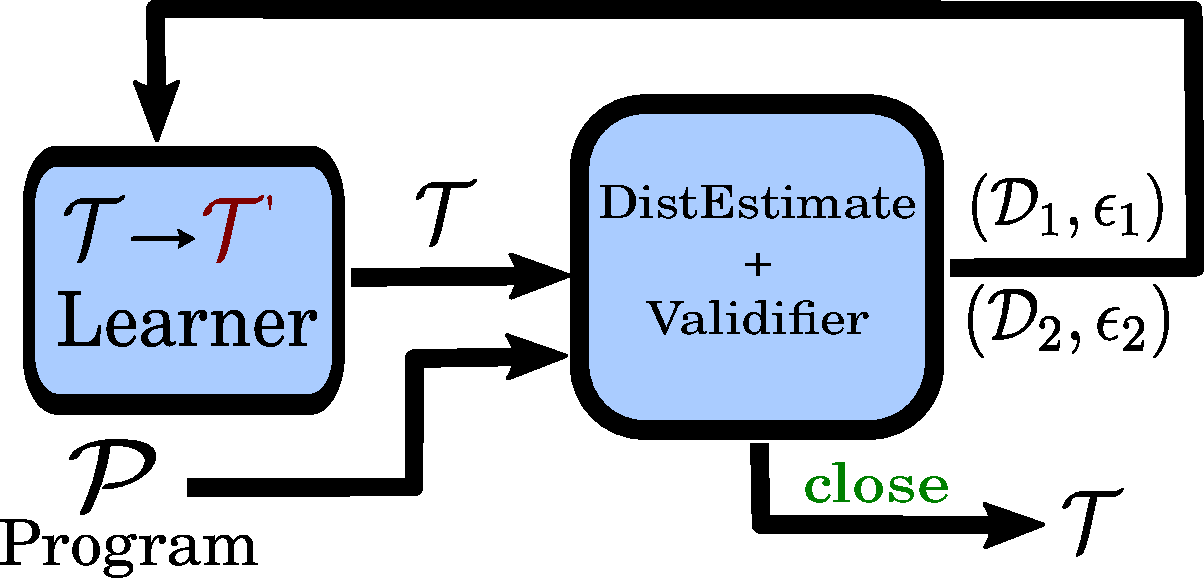
\includegraphics[scale=0.5]{assets/archi.pdf}
		\caption{Overview}
		\label{fig:overview}
	\end{figure}


The \textit{DistEstimate} and \textit{Validifier} modules will return the pairs (\distdata, $\epsilon_1$) and (\validata, $\epsilon_2$) respectively (see \cref{fig:overview}). 

Assuming dataset $\text{\distdata }$ contains $n_1$ data points $\{(s_i, w_i, l_i)\}_{i=1}^{n_1}$,  where $s_i$ denotes a program state, $w_i$ denotes its weight and $l_i \in \{0,1\}$ is a label; $l_i$ is 0 if the state $s_i \not \models \text{\candidate}$ and $l_i$ is 1 if $s_i \models \text{\candidate}$. We also use $l_i^{ex}$ to denote the expected labels of the states, for $s_i \in \text{\distdata}$, $l_i^{ex}$ is 1.
\sepa
\begin{tcolorbox}[colback=lightgray!10!white, colframe=black!30!black,title=Error Probability $\epsilon_1$ , sharp corners, width=\textwidth, boxsep=1pt]
	\centering
	Any random sampled state from $S$, must reach \candidate with probability ($1 - \epsilon_1$) in K-steps
\end{tcolorbox}
\sepa
Similarly, assume dataset $\text{\validata }$ contains $n_2$ data points $\{(s_i, l_i)\}_{i=1}^{n_2}$, where $s_i$ denotes a program state and $l_i \in \{0,1\}$. In this case, $l_i = 0$ if $s_i$ is not reachable from $S$ otherwise $l_i = 1$. We also use $l_i^{ex}$ to denote the expected labels of the states, for $s_i \in \text{\validata}$, $l_i^{ex} = l_i$.
\sepa
\begin{tcolorbox}[colback=lightgray!10!white, colframe=black!30!black,title=Error Probability $\epsilon_2$ , sharp corners, width=\textwidth, boxsep=1pt]
	\centering
	Any random sampled state from \candidate, must be reachable from $S$ in K-steps with probability ($1 - \epsilon_2$).
\end{tcolorbox}


\paragraph{\textbf{Cases to consider while mutating:}}
\begin{enumerate}
	\item $\forall s_i \in \text{\distdata}$ with $l_i = 1$, we want to preserve the label of such states in $\mathcal{T}'$.
	\item  $\forall s_i \in \text{\distdata}$ with $l_i = 0$, we want to include these states in $\mathcal{T}'$ i.e. flip the labels of such states.
	\item $\forall s_i \in \text{\validata}$ with $l_i = 1$, we want to preserve the label of such states in $\mathcal{T}'$.
	\item $\forall s_i \in \text{\validata}$ with $l_i = 0$, we want to exclude such states from $\mathcal{T}'$.
\end{enumerate}

\paragraph{\textbf{Mutations.}}
If $\text{\candidate }$ has x leaves then maximum possible mutations are $2 \cdot x$. For each leaf following two mutations are possible:
\begin{enumerate}
	\item Splitting a leaf node.
	\item Pruning a leaf node.
\end{enumerate}

\paragraph{\textbf{Cost of Mutations.}}
Pruning a leaf node is preferred over splitting therefore cost of pruning should be less than the cost of splitting the node. For both types of mutations, mutating a leaf at higher depth is preferred than a leaf at lower depth therefore cost of applying any mutation on a leaf at higher depth is lesser than applying mutation on a leaf at lower depth.

\section{Problem Statement}

Given \candidate and the pairs (\distdata, $\epsilon_1$) and (\validata, $\epsilon_2$), make minimal mutations to $\text{\candidate }$ to obtain a $\mathcal{T}'$ such that following two inequalities hold:

\begin{align}
	& \sum_{s_i \in \mathcal{D}_1}(w_i \cdot (|l_i^{\text{ \candidate}'} - l_i^{ex}|)) \leq \text{\userrdist}  \label{eq:disterror}& \\
	& \frac{\sum_{s_i \in \mathcal{D}_2}(1 \cdot (|l_i^{\text{ \candidate}'} - l_i^{ex}|))}{n_2} \leq \text{\userrvalid} \label{eq:validerror} &
\end{align}


\section{Algorithm}

Given a candidate $\text{\candidate}$, pairs (\distdata, $\epsilon_1$) and (\validata, $\epsilon_2$) and user supplied error bounds \userrdist and \userrvalid, \cref{algo:first} mutates \candidate and outputs $\text{\candidate}'$ such that \cref{eq:disterror} and \cref{eq:validerror} are satisfied.

\textbf{extractLeaves.} Returns a mapping of states in $\text{\distdata}$ and $\text{\validata}$ to leaves indices of the tree \candidate as a dictionary.



\begin{algorithm}
	\caption{getGain($\text{\candidate}, l, m, \epsilon_1, \epsilon_2$)}
	\label{algo:gain}
	\begin{algorithmic}[1]
		\State $\text{\candidate}' \gets Mutate(\text{\candidate})$
		\State $\epsilon_1', \epsilon_2' \gets getEstimates(\text{\candidate}') \text{\hspace{0.1 in}//Using \cref{eq:disterror} and \cref{eq:validerror}}$
		\State $gain \gets (\epsilon_1 - \epsilon_1') + (\epsilon_2 - \epsilon_2')$
		\State $return \text{ } gain, \epsilon_1', \epsilon_2'$		
	\end{algorithmic}
\end{algorithm}


\begin{algorithm}
	\caption{getCost($dep, m$)}
	\label{algo:cost}
	\begin{algorithmic}[1]
		\State $return \text{ } 1$		
	\end{algorithmic}
\end{algorithm}



\begin{algorithm}
	\caption{MuteTree(\candidate, \distdata, \validata, $\epsilon_1$, $\epsilon_2$, \userrdist, \userrvalid)}
	\label{algo:first}
	\begin{algorithmic}[1]
		\State $\epsilon_1', \epsilon_2' \gets 0, 0$
		\While{$\epsilon_1' \leq \text{\userrdist} \land \epsilon_2' \leq \text{\userrvalid}$}
		\State $moves, leaves \gets [], \{\} $
		\State $ leaves \gets extractLeaves(\text{\candidate}, \text{\validata}, \text{\distdata})$
		\For{$l \in leaves$}
		\For{$m \in mutations$}
		\State $gain, \text{\candidate}', \epsilon_1', \epsilon_2' \gets getGain(\text{\candidate}, l, m, \epsilon_1, \epsilon_2)$
		\State $cost \gets getCost(depth(l), m)$
		\State $ratio \gets \frac{gain}{cost}$
		\State $moves.append((ratio, \text{\candidate}', \epsilon_1', \epsilon_2'))$
		\EndFor
		\EndFor
		\State $moves \gets sort(moves, key=ratio)[:k]$
		\State $moves \gets normalize(moves, key=ratio)$
		\State $\text{\candidate}', \epsilon_1', \epsilon_2' \gets SampleUniform(moves)$
		\EndWhile
		\State $return \text{ \candidate}'$
	\end{algorithmic}
\end{algorithm}






\clearpage


%\begin{tikzpicture}[level distance=1.5cm,
%	level 1/.style={sibling distance=5cm},
%	level 2/.style={sibling distance=3cm},
%	level 3/.style={sibling distance=2cm}]
%	
%	% Root node
%	\node {Predicate}
%	% Level 1
%	child {node {Predicate}
%			% Level 2
%			child {node {Predicate}
%					% Level 3 leaves with mixed blue and red points
%					child {node [draw, rectangle, minimum width=0.7cm, minimum height=0.7cm] {
%									\textcolor{blue}{$\bullet$} \textcolor{red}{$\bullet$} \textcolor{blue}{$\bullet$}}}
%					child {node [draw, rectangle, minimum width=0.7cm, minimum height=0.7cm] {
%									\textcolor{red}{$\bullet$} \textcolor{red}{$\bullet$} \textcolor{red}{$\bullet$}}}
%				}
%			child {node {Predicate}
%					% Level 3 leaves with mixed blue and red points
%					child {node [draw, rectangle, minimum width=0.7cm, minimum height=0.7cm] {
%									\textcolor{blue}{$\bullet$} \textcolor{red}{$\bullet$}}}
%					child {node [draw, rectangle, minimum width=0.7cm, minimum height=0.7cm] {
%									\textcolor{red}{$\bullet$} \textcolor{blue}{$\bullet$} \textcolor{red}{$\bullet$}}}
%				}
%		}
%	child {node {Predicate}
%			% Level 2
%			child {node {Predicate}
%					% Level 3 leaves with mixed blue and red points
%					child {node [draw, rectangle, minimum width=0.7cm, minimum height=0.7cm] {
%									\textcolor{red}{$\bullet$} \textcolor{red}{$\bullet$} \textcolor{red}{$\bullet$}}}
%					child {node [draw, rectangle, minimum width=0.7cm, minimum height=0.7cm] {
%									\textcolor{blue}{$\bullet$} \textcolor{red}{$\bullet$} \textcolor{blue}{$\bullet$}}}
%				}
%			child {node {Predicate}
%					% Level 3 leaves with mixed blue and red points
%					child {node [draw, rectangle, minimum width=0.7cm, minimum height=0.7cm] {
%									\textcolor{blue}{$\bullet$} \textcolor{blue}{$\bullet$} \textcolor{red}{$\bullet$}}}
%					child {node [draw, rectangle, minimum width=0.7cm, minimum height=0.7cm] {
%									\textcolor{red}{$\bullet$} \textcolor{blue}{$\bullet$} \textcolor{blue}{$\bullet$}}}
%				}
%		};
%\end{tikzpicture}





\end{document}